%%%%%%%%%%%%%%%%%%%%%%%%%%%%%%%%%%%%%%%%%%%%%%%%%%%%%%%%%%%%%%%%%%
\section{Procesado de los datos}
\label{sec:preprocesado}

En las Secciones anteriores, se ha detallado el proceso de búsqueda y recolección de datos energéticos en entornos residenciales a partir de las fuentes públicas disponibles. Este proceso ha venido acompañado por un estudio y análisis en profundidad para exponer de forma justificada las razones de la selección de los conjuntos de datos que servirán como base de este \gls{tfm}. 

\vspace{3mm}

También, se ha llevado a cabo una investigación enfocada en dos herramientas de extracción de información geográfica, climática y energética. El fin de este proceso ha sido incorporar una nueva fuente de datos con parámetros relacionados con la producción de electricidad, la cual se ha construido a partir de la simulación de un caso real.

\vspace{3mm}

Entonces, se puede expresar que la ejecución de los procesos anteriores proporcionará múltiples ficheros de datos que soporten extensas cantidades de información. En consecuencia, estos ficheros se caracterizarán por su gran tamaño y su dificultad de manejo y empleo. Por ello, se introduce esta Sección con el fin principal de realizar un procesamiento exhaustivo y reducir los conjuntos de datos únicamente a las muestras que aporten información de utilidad para llevar a cabo el desarrollo posterior. Teniendo en cuenta el objetivo definido, se va a estructurar esta Sección en diferentes fases, en función de cada uno de los pasos que se deberán realizar para procesar los datos.

\vspace{3mm}

Antes de comenzar a describir este procesamiento, es imprescindible destacar que este vendrá determinado principalmente por la creación y diseño de código programado en \textit{Python} en diferentes \textit{notebooks} de \textit{Jupyter}, ya que es el entorno más adecuado en el ámbito de la ciencia de datos y de la aplicación de técnicas de \gls{ml}. Su empleo aportará la ventaja de poder depurar y comprobar paso a paso que se ejecutan de forma correcta cada una de las acciones que componen el procesamiento. Además, cabe destacar el uso de algunas librerías que serán imprescindibles para el manejo de los datos, como son \textit{pandas}, \textit{csv} o \textit{numpy}, entre otras.

\subsection{Procesado de datos de consumo}

\subsubsection{Análisis de la situación inicial y primeros pasos}
\label{sec:inicialproc}

El dataset seleccionado para este \gls{tfm}, \textit{SustDataED}, se detallaba en la Sección \ref{sec:sustdataed} como un conjunto de datos que abría multitud de posibilidades de implementación. Se puede expresar que esto venía justificado por el hecho de abarcar un extenso lapso temporal de medidas correspondientes a un gran número de viviendas. Además, estas medidas se caracterizaban por ser adquiridas a una frecuencia de muestreo de un minuto, lo que aportaba una buena resolución para analizar el comportamiento eléctrico de todos los usuarios implicados. 

\vspace{3mm}

Como también se exponía en la Sección \ref{sec:sustdataed}, especialmente en la Figura \ref{fig:despliegues}, el dataset \textit{SustDataED} se estructuraba en cuatro despliegues diferentes, cada uno con diferentes rangos temporales de medición y con un conjunto de viviendas determinado. Poniendo el enfoque en las medidas de consumo, esto supone que se termine coleccionando en conjunto hasta un total de 24.512.181 muestras, correspondientes a 1144 días de medición. A modo de síntesis, se aporta la Tabla \ref{tab:resumen} con la información respectiva a cada despliegue. \cite{sustdata}

\vspace{3mm}

\begin{table}[h!]
    \centering
    \begin{tabular}{c|c|c|cc}
    \hline
    \rowcolor[HTML]{C0C0C0} 
    \multicolumn{1}{|l|}{\cellcolor[HTML]{C0C0C0}Despliegue} & \multicolumn{1}{l|}{\cellcolor[HTML]{C0C0C0}Muestras} & \multicolumn{1}{l|}{\cellcolor[HTML]{C0C0C0}Días} & \multicolumn{1}{l|}{\cellcolor[HTML]{C0C0C0}Fecha de inicio} & \multicolumn{1}{l|}{\cellcolor[HTML]{C0C0C0}Fecha de fin} \\ \hline
    \multicolumn{1}{|c|}{1} & 3.474.557 & 123 & \multicolumn{1}{c|}{10/07/2010} & \multicolumn{1}{c|}{10/11/2010} \\ \hline
    \multicolumn{1}{|c|}{2} & 12.481.536 & 504 & \multicolumn{1}{c|}{25/11/2010} & \multicolumn{1}{c|}{20/04/2012} \\ \hline
    \multicolumn{1}{|c|}{3} & 5.671.576 & 298 & \multicolumn{1}{c|}{01/08/2012} & \multicolumn{1}{c|}{25/05/2013} \\ \hline
    \multicolumn{1}{|c|}{4} & 2.884.512 & 219 & \multicolumn{1}{c|}{31/07/2013} & \multicolumn{1}{c|}{10/03/2014} \\ \hline
    \multicolumn{1}{l|}{} & \multicolumn{1}{l|}{\cellcolor[HTML]{EFEFEF}24.512.181} & \multicolumn{1}{l|}{\cellcolor[HTML]{EFEFEF}1144} & \multicolumn{1}{l}{} & \multicolumn{1}{l}{} \\ \cline{2-3}
    \end{tabular}
    \caption{Resumen de los datos de consumo del dataset \textit{SustDataED} \cite{sustdata}}
    \label{tab:resumen}
\end{table}

\vspace{3mm}

Tomando lo anterior en consideración, en este paso, enfocado al análisis de la situación inicial del conjunto, es preciso tener el conocimiento de los ficheros de datos de consumo de los que se va a partir. Por este motivo, se añade de forma adicional la Tabla \ref{tab:fichconsumo}, la cual expone la información relativa a cada despliegue y a los tamaños de cada uno de los ficheros proporcionados en el dataset.  

\vspace{3mm}

\begin{table}[h!]
    \centering
    \begin{tabular}{|c|c|c|}
    \hline
    \rowcolor[HTML]{C0C0C0}
    \multicolumn{1}{|l|}{\cellcolor[HTML]{C0C0C0}Despliegue} & Fichero de muestras & \multicolumn{1}{l|}{\cellcolor[HTML]{C0C0C0}Tamaño (MB)} \\
    \hline
    1 & power\_samples\_d1\_1 & 86.38 \\
      & power\_samples\_d1\_2 & 69.99 \\
    \hline
    2 & power\_samples\_d2\_1 & 289.81 \\
      & power\_samples\_d2\_2 & 265.13 \\
      & power\_samples\_d2\_3 & 283.27 \\
      & power\_samples\_d2\_4 & 311.89 \\
    \hline
    3 & power\_samples\_d3\_1 & 259.92 \\
      & power\_samples\_d3\_2 & 233.69 \\
      & power\_samples\_d3\_3 & 272.23 \\
    \hline
    4 & power\_samples\_d4\_1 & 250.12 \\
      & power\_samples\_d4\_2 & 252.84 \\
    \hline
    \end{tabular}
    \caption{Resumen de las características de los ficheros de los despliegues de \textit{SustDataED}}
    \label{tab:fichconsumo}
\end{table}

\vspace{3mm}

Como se puede comprobar, a priori la mayoría no precisan de un volumen manejable, por lo que la primera acción a realizar será dividir los mismos en nuevos ficheros que supongan un tamaño menor del dado. Esto sobre todo será importante a la hora de trabajar con el repositorio de GitHub, puesto que existe el factor limitante de que el tamaño máximo permitido por archivo es de 100MB. 

\vspace{3mm}

No obstante, antes de dividir los ficheros, se debe volver a la Tabla que hace referencia a las medidas de consumo energético (ver Tabla \ref{tab:consumo}) para observar que estos ficheros contienen una columna dedicada a la marca de tiempo (\textit{timestamp}) del instante en el que se adquirió la medida. A modo de simplificar esta información temporal, se crea el \textit{notebook} \textit{preprocessing\_nodes.ipynb}, que va a importa la librería \textit{time} para añadir tres nuevas columnas al dataset que separen los datos de la fecha (columna \textit{datetime}), el instante exacto de la muestra (hora, minuto y segundo) (columna \textit{hour}) y la hora como un valor entero (columna \textit{H}). En el caso de esta última columna, su utilidad vendrá descrita por los requerimientos de la siguiente Sección (ver Sección \ref{sec:datasamples}).

\vspace{3mm}

\begin{lstlisting}[style=Python-color, caption={Formato del timestamp}]
  df['tmstp'] = pd.to_datetime(df['tmstp']) # Conversión de la columna del \textit{dataframe} a formato datetime
  df['datetime'] = df['tmstp'].dt.strftime('%Y-%m-%d') # Formateo de la fecha (año, mes, día)
  df['hour'] = df['tmstp'].dt.strftime('%H:%M:%S') # Formateo del instante (hora, minuto, segundo)
  df['H'] = df['tmstp'].dt.strftime('%H').astype(int) # Formateo de la hora como entero
\end{lstlisting}

\vspace{3mm}

De forma adicional, en este \textit{notebook} se comprueba también, si existen filas con valores \textit{NaN} que puedan perjudicar al análisis de los datos. Como ventaja, el dataset \textit{SustDataED} aporta la columna \textit{miss\_flag} (ver Tabla \ref{tab:consumo}) para determinar si para cierto instante temporal se ha producido la adquisición de forma incorrecta o con valores vacíos. Por tanto, la acción a desarrollar será comprobar en todo el \textit{dataframe} cuándo este valor se encuentra activo y, en ese caso, eliminar la fila respectiva.

\vspace{3mm}

\begin{lstlisting}[style=Python, caption={Eliminación de valores NaN}]
  df.isnull().any() # Comprobación previa de existencia de valores NaN en el \textit{dataframe}
  df = df[df['miss_flag'] != 1] # Aplicación de filtro al \textit{dataframe}
  df = df.dropna(thresh=len(df.columns) - 15 + 1) # Eliminación de columnas con todos los elementos vacíos
  df.isnull().any() # Comprobación posterior de existencia de valores NaN en el \textit{dataframe}
\end{lstlisting}

\vspace{3mm}

A modo de resumen, se puede determinar entonces, que se seguirá la siguiente secuencia de pasos en esta primera fase: crear las nuevas columnas temporales, eliminar las filas que estén completamente vacías y dividir los ficheros iniciales para ajustar su tamaño a un máximo de 100MB. Es obligatorio seguir este orden, puesto que no sería eficiente extraer los fragmentos del conjunto de datos y, después, añadir información nueva. En otros términos, de esta forma se estaría superando el tamaño máximo ajustado en los nuevos ficheros de salida.

\vspace{3mm}

Volviendo al proceso de división de los ficheros, se crea otro \textit{notebook} de \textit{Jupyter}, denominado como \textit{split.ipynb}. En primer lugar, se importa al mismo la librería de \textit{Python} \textit{csv}, enfocada al tratamiento de archivos con formato .csv. Después, se escribe una función que, a partir de un fichero de entrada, itere a través de sus filas de datos hasta llegar al volumen máximo determinado para obtener a la salida el nuevo archivo en la ruta indicada. Además, para cada nueva fragmentación de los datos se incluye el encabezado con los nombres de cada uno de los campos.

\vspace{3mm}

\begin{lstlisting}[style=Python, caption={Fragmentación de ficheros iniciales}]
  with open(input_file, 'r') as csv: # Apertura del fichero de entrada
    reader = csv.reader(csv) # Definición del reader
    header = next(reader)  

  for row in reader: # Iteración de las filas del fichero
      if current_row % split_size == 0:  # Condición de máximo de filas
          if output_file: # Cierre del fichero de salida 
              output_file.close()
          split = f'dataset/split_{current_split}.csv'
          output_name = input_name + split
          output_file = open(output_name, 'w', newline='') # Apertura del fichero de salida
          writer = csv.writer(output_file) # Definición del writer
          writer.writerow(header) # Escritura del encabezado
          current_split += 1
      writer.writerow(row) # Escritura de fila
      current_row += 1

if output_file: # Cierre del fichero de salida
  output_file.close()
\end{lstlisting}

\vspace{3mm}

Por tanto, tras realizar este procedimiento, se logra obtener un total de 28 nuevos ficheros en formato .csv de un tamaño reducido, permitiéndose así, una mejor gestión de los datos que contienen los mismos.

\subsubsection{Síntesis de la información}
\label{sec:datasamples}

La presente Sección se dedicará principalmente a la reducción de la información dada por \textit{SustDataED}. Como se ha comentado anteriormente, el hecho de que las muestras se hayan adquirido a una frecuencia de un minuto, proporciona un gran volumen de datos que debería sintentizarse. En el caso de este \gls{tfm}, con el fin de reducir el número de filas del dataset, se ha valorado como opción más apropiada realizar una cuantificación del promedio de las mediciones para cada hora. En otros términos, a partir de las muestras iniciales obtenidas cada minuto, se generaría un nuevo conjunto de medidas promediadas cada hora, resultando en una reducción de los datos en un factor 60.

\vspace{3mm}

En primera instancia, para simplificar la programación, se crea un primer \textit{notebook} básico que realice el procedimiento de reducción de datos para uno de los ficheros fragmentados que se han obtenido a partir de \textit{split.ipynb}. Este nuevo \textit{notebook} se denomina como \textit{datasamples\_onenode.ipynb} y aplica el promedio únicamente a las medidas de un nodo contenidas en una hora y fecha determinadas. Estos valores son determinados como parámetros de entrada y, en el caso de la hora, es preciso hacer uso de la columna \textit{H}, definida en la Sección anterior (ver Sección \ref{sec:inicialproc}) para determinar la hora a la que pertenece la medida como un valor entero.

\vspace{3mm}

Por tanto, una vez definidos los valores de los parámetros de entrada, se aplica un filtro al \textit{dataframe} a partir de los mismos y se comprueba que se ha realizado el procedimiento de forma correcta mediante la observación del número de filas que se extraen, que debería ser 60. Para llevar a cabo el cálculo del promedio, es preciso especificar las columnas sobre las que se va a aplicar la operación, que son las que contienen todos los valores que hacen referencia a los parámetros eléctricos. Por tanto, a partir de las 60 filas filtradas y, tomando en consideración las columnas comentadas, se puede calcular ya el valor promedio de cada uno de los parámetros eléctricos. 

\vspace{3mm}

El resultado de este proceso supone una única fila con todos los valores promediados de una hora. En la Figura \ref{fig:datasamples} se muestra como ejemplo la salida que se obtiene tras aplicar el promedio a las medidas adquiridas en la vivienda con identificador 25 en el instante temporal correspondiente al 8 de abril de 2013 con hora 15:00.

\vspace{3mm}

\begin{figure}[h!]
  \centering
  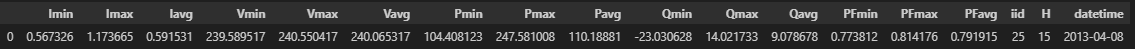
\includegraphics[width=1\textwidth]{img/diseno/datasamples.png}
  \caption{Salida de \textit{datasamples\_onenode.ipynb} tras aplicar la operación de promedio}
  \label{fig:datasamples}
\end{figure}

\subsubsection{Automatización del proceso de síntesis de la información}
\label{sec:datasamples}

Como se viene exponiendo en la Sección anterior (ver Sección \ref{sec:datasamples}), el proceso de cálculo del promedio de valores viene determinado por los parámetros de entrada que se definen y se produce una ejecución únicamente para las 60 muestras que se han adquirido a partir de un identificador de vivienda y en una hora y fecha específicas. 

\vspace{3mm}

Esta característica supone que, si se desea aplicar el promedio a los valores de las medidas de cada hora para todo el rango temporal que abarca cada uno de los nodos, se debe automatizar el proceso. Por ello, se crea un nuevo archivo de \textit{Python}, denominado como \textit{datasamples\_process.py}, que incluirá todas las funciones necesarias para llevar a cabo el procedimiento de automatización. 

\vspace{3mm}

Es importante comentar que en esta Sección se pone el foco en los datos de consumo. Sin embargo, las funciones que se van a exponer a continuación, serán configuradas para ser empleadas también, en el caso de los datos relativos a la producción y al clima de \textit{SustDataED}.

\vspace{3mm}

En primer lugar, \textit{datasamples\_process.ipynb} describe una función de lectura que extrae como argumento el \textit{path} donde se ubican los ficheros .csv a leer y, después, aplica un bucle para concatenar todos ellos en un mismo \textit{dataframe}. Por consiguiente, se comprueba qué tipo de datos contienen los ficheros (ficheros de consumo o de producción) y se almacenan las columnas de los parámetros eléctricos con los que se va a operar en una variable X. En el caso de los ficheros de consumo, se selecciona la columna \textit{Pavg}, que hace referencia a los valores de potencia activa media adquirida en cada instante. Esto es porque se trata de la información que se requiere conocer para poder establecer más adelante las cargas en el algoritmo \gls{den2ne}. Este proceso en cuestión será detallado en la Sección \ref{sec:cambiosden2ne}.

\vspace{3mm}

En el paso de lectura se extraen también los identificadores de las viviendas que vienen contenidos en cada fichero. Finalmente, se devuelve el \textit{dataframe} completo, la variable X y dos listas: una con los identificadores extraídos en el paso anterior y otra con todas las fechas únicas (columna \textit{datetime}) que contiene el \textit{dataframe}.

\vspace{3mm}

\begin{lstlisting}[style=Python, caption={Función de lectura de los ficheros}]
  def read_files(files):
      path = gl.glob(files) # Definición del path
      dfs = []

      for file in path:
          dfs.append(pd.read_csv(file, low_memory=False)) # Lectura de cada fichero
          print("Leyendo " + file)

      df = pd.concat(dfs, ignore_index=True) # Operación de concatenación

      # Comprobación de tipo de ficheros para almacenar los parámetros eléctricos y los identificadores
      if files.startswith(files_cons): # Ficheros de consumo
          X = df.iloc[:, 11:12]
          iid_array = df["iid"].unique()
      elif files == files_prod: # Ficheros de producción
          X = df.iloc[:, 16:17]
          iid_array = 0

      X_features = X.columns.to_list()
      X_features.append("iid")
      X_features.append("datetime")
      X_features.append("h")
      datetime_array = df["datetime"].unique() # Extracción de las fechas
      return df, X_features, iid_array, datetime_array
\end{lstlisting}

\vspace{3mm}

La siguiente función que se define es la relativa al cálculo del promedio de los valores. En ella, al igual que en la anterior, es preciso comprobar si los ficheros con los que se va a operar contienen datos de consumo o de producción. Se aplica una condición para ello a partir de la existencia de información sobre el identificador de la vivienda, ya que, como se comentaba en la Sección \ref{sec:prodsustdata}, los datos de producción de \textit{SustDataED} se proporcionan en términos globales a todos los hogares. Esto quiere decir que no proveen información de identificador, por lo que es posible conocer el tipo de ficheros que se está tratando a partir del valor de esta columna.

\vspace{3mm}

Por tanto, tomando lo anterior en consideración, se aplica el filtro al \textit{dataframe} de la misma forma que se realizaba en la Sección \label{sec:datasamples} y se informa, a modo de depuración, sobre el progreso del proceso. El siguiente paso es calcular la media de los valores para cada hora y volcar los resultados, junto con el identificador de la vivienda y el dato de la fecha, en un nuevo \textit{dataframe}.

\vspace{3mm}

\begin{lstlisting}[style=Python, caption={Función de cálculo del promedio}]
  def extract_mean(df, IID_SAMPLE, HOUR_SAMPLE, DATETIME_SAMPLE, X_features, result_dict, progress):
      # Comprobación de tipo de ficheros para aplicar el filtro
      if IID_SAMPLE == 0: # Ficheros de producción
          filter = df[(df["h"] == HOUR_SAMPLE) & (df["datetime"] == DATETIME_SAMPLE)]
          desc = f"Procesando producción {DATETIME_SAMPLE} {HOUR_SAMPLE}"
      else: # Ficheros de consumo
          filter = df[(df["iid"] == IID_SAMPLE) & (df["h"] == HOUR_SAMPLE) 
          & (df["datetime"] == DATETIME_SAMPLE)]
          desc = f"Procesando consumo de IID {IID_SAMPLE} {DATETIME_SAMPLE} {HOUR_SAMPLE}"

      df2 = pd.DataFrame() # Creación del nuevo \textit{dataframe} para almacenar los resultados

      for feature in X_features:
          if feature == "iid":
              df2[feature] = IID_SAMPLE
          elif feature == "datetime":
              df2[feature] = DATETIME_SAMPLE
          else:
              df2[feature] = [filter[feature].mean()] # Cálculo del promedio

      result_dict[IID_SAMPLE] = df2 # Diccionario final con todos los \textit{dataframes} creados
      progress.value += 1
\end{lstlisting}

\vspace{3mm}

Finalmente, se escribe la función que se va a encargar de automatizar el proceso de cálculo de todos los valores promedios mediante compresión de listas. Se produce la llamada a la función \textit{extract\_mean()} con un doble bucle que introduce iteraciones en función de todas las fechas contenidas en la lista de fechas y de todas las horas que hay en un día.

\vspace{3mm}

\begin{lstlisting}[style=Python, caption={Función de automatización del cálculo del promedio}]
  def process_data(iid, df_power_samples, datetime_array_ps, X_ps, result_dict, progress):
    extraction = [
        extract_mean(df_power_samples, iid, hour, datetime, X_ps, result_dict, progress)
        for datetime in datetime_array_ps
        for hour in range(24)]
\end{lstlisting}

\vspace{3mm}

%la cual se lleva a cabo desde los ordenadores del laboratorio
Por lo tanto, una vez definidas las funciones anteriores, ya se permite realizar una ejecución automatizada del proceso de síntesis de los datos. En este caso, para realizar las pruebas de funcionamiento, se crea el script \textit{run\_tests.sh} y se lanza en un equipo que cuenta con un total de 32 cores. Este script posibilita la descompresión de los ficheros de datos, la instalación de las librerías de \textit{Python} necesarias (especificadas en un archivo \textit{requirements.txt}) y la ejecución de \textit{datasamples\_process.ipynb}.

\vspace{3mm}

% \begin{lstlisting}[language=bash, style=Consola, caption={Script para el lanzamiento de las pruebas}]
%   #!/bin/bash

%   dir_zip="zipped/"
%   dir_dest="unzipped/"
%   dir_results="results/"
  
%   pip freeze > "before.txt" 
  
%   if [ -f requirements.txt ]; then
%       echo "Instalando paquetes"
%       pip install -r requirements.txt
%       echo "Instalación completada"
%       #pip freeze > "after.txt" 
%   else
%       echo "El archivo requirements.txt no existe"
%   fi
  
%   if [ ! -d "$dir_dest" ]; then
%       echo "Creando directorio destino unzipped/"
%       mkdir -p $dir_dest
%   else
%       echo "Existe $dir_dest"
%   fi
  
%   if [ ! -d "$dir_results" ]; then
%       echo "Creando directorio destino results/"
%       mkdir -p $dir_results
%   else
%       echo "Existe $dir_results"
%   fi
  
%   if [ ! -d "$dir_zip" ]; then
%       echo "No existe $dir_zip" 
%   else
%       ls $dir_zip
%       if [ "$(ls -A $dir_dest)" ]; then
%           echo "Descompresión ya realizada anteriormente"
%       else
%           unzip $dir_zip"*.zip" -d $dir_dest
%           echo "Descompresión completada" 
%       fi 
%   fi
  
%   if [ -f datasamples.py ]; then
%       echo "-----------------------------------------------------"
%       echo "Ejecutando archivo"
%       echo "-----------------------------------------------------"
%       python3 datasamples.py 
%   else
%       echo "El archivo datasamples.py no existe"
%   fi
  
%   echo "Ejecución completada"
  
%   pip uninstall -r requirements.txt
%   pip freeze > "before2.txt" 
%   diff before.txt before2.txt
% \end{lstlisting}

% \vspace{3mm}

Se plantea en primera instancia, establecer una ejecución multihilo. Cuando se lleva a cabo el lanzamiento, se observa que, como es de esperar, se están utilizando varios cores. Sin embargo, como se puede visualizar en la Figura \ref{fig:multihilo}, el uso de \textit{threads} no provoca en ningún momento que alguno de los cores disponibles se aproxime al 100\% de su operabilidad.

\vspace{3mm}

\begin{figure}[h!]
  \centering
  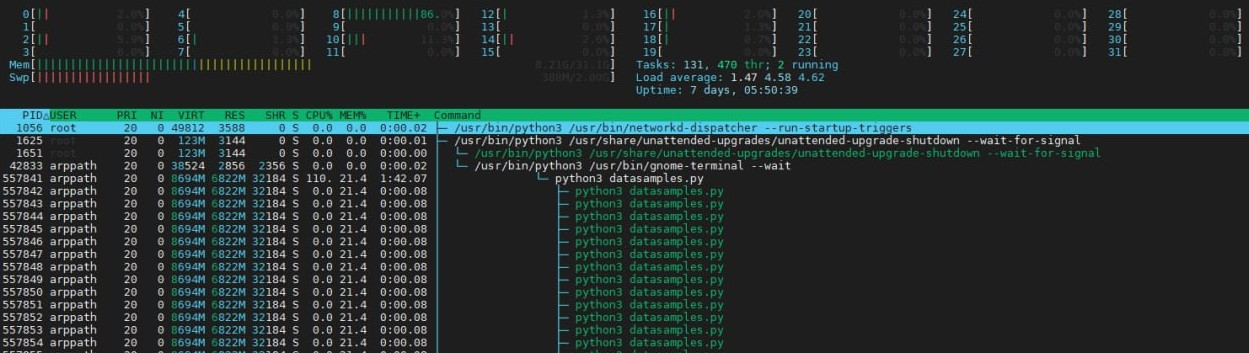
\includegraphics[width=1\textwidth]{img/diseno/multihilo.jpg}
  \caption{Lanzamiento de pruebas con \textit{threads}}
  \label{fig:multihilo}
\end{figure}

\vspace{3mm}

Esto se debe a que los hilos no son procesos y están principalmente enfocados a la concurrencia. Es decir, el planificador del kernel establece en qué core se va a ejecutar cada una de las tareas y se producen cambios de contexto, que tienen como consecuencia, la introducción de latencias y una pérdida de eficiencia en la ejecución de las pruebas. Teniendo esto en cuenta, se toma la decisión de operar con procesos independientes. En este caso, no se van a producir desalojos, dado que la tarea sí es un proceso. Además, se establece uno para cada identificador, suponiendo que cada uno de ellos se ejecute completamente en un core. En la Figura \ref{fig:multiprocess}, se muestran los cambios comentados. \cite{thread}

\vspace{3mm}

\begin{figure}[h!]
  \centering
  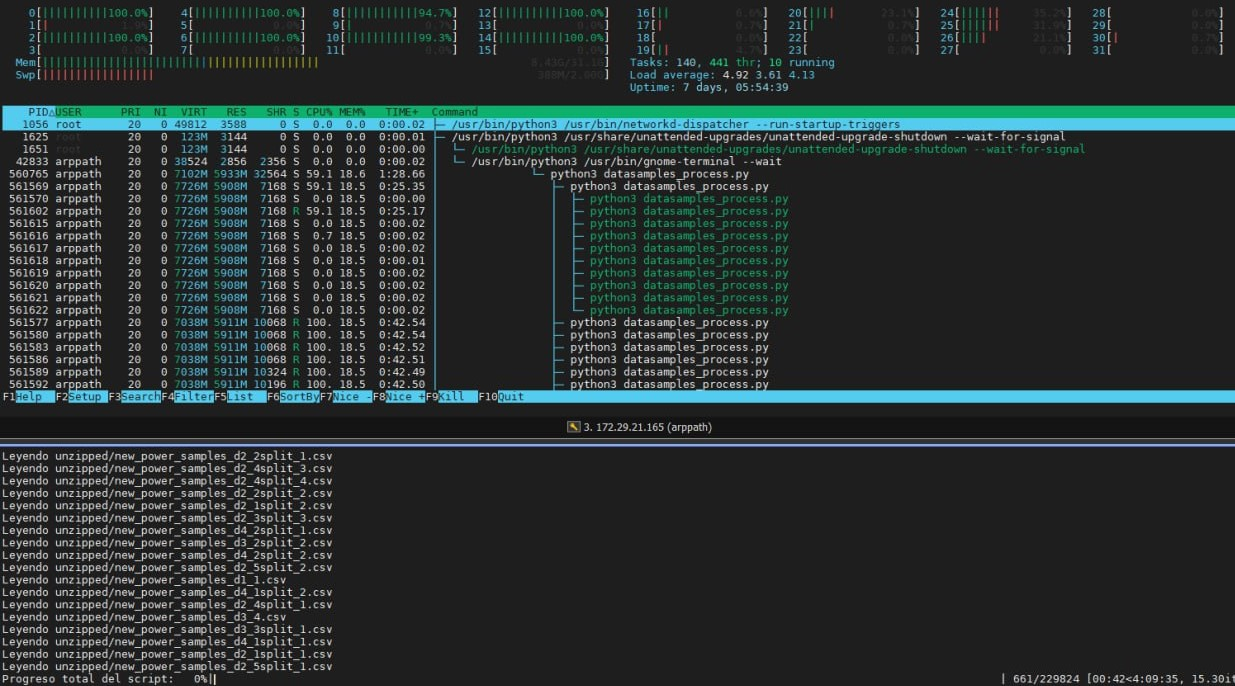
\includegraphics[width=1\textwidth]{img/diseno/multiprocess.jpg}
  \caption{Lanzamiento de pruebas con procesos}
  \label{fig:multiprocess}
\end{figure}

\vspace{3mm}

Por lo tanto, volviendo al código, en el archivo se debe importar la librería \textit{multiprocessing} y definir el administrador (\textit{manager}) para crear un diccionario que será compartido por los procesos para almacenar los resultados de la ejecución. Después, se crean los procesos, llamando a la función \textit{process\_data}, expuesta anteriormente. Para la misma, se deben añadir los parámetros de entrada necesarios como argumentos e iterar para todos los identificadores de viviendas. En este momento, ya se pueden iniciar los procesos y definir el progreso de la ejecución a través de la terminal. 

\vspace{3mm}

\begin{lstlisting}[style=Python, caption={Creación de procesos}]
  if __name__ == "__main__":
  df_power_samples, X_ps, iid_array_ps, datetime_array_ps = read_files(files_cons) # Lectura de ficheros

  manager = Manager() # Creación del administrador
  result_dict = manager.dict() # Definición del diccionario compartido de resultados
  progress = manager.Value('i', 0) # Creación de valor para indicar el progreso

  processes = [   # Creación de los procesos
      Process(target=process_data, args=(iid, df_power_samples, datetime_array_ps, X_ps, result_dict, progress))
      for iid in iid_prueba
  ]

  for process in processes: 
      process.start() # Inicio de los procesos

  total_tasks = len(datetime_array_ps) * len(iid_prueba) * 24 # Cálculo del número de tareas

  # Creación de barra de progreso
  with tqdm(total=total_tasks, desc="Progreso total del script") as pbar:
      while progress.value < total_tasks:
          pbar.update(progress.value - pbar.n)

  for process in processes:
      process.join() # Espera a la finalización de todos los procesos

  for iid, result in result_dict.items(): # Almacenamiento de los resultados en los nuevos ficheros
      result.to_csv(f"results/consum_{iid}.csv", index=False) 
\end{lstlisting}

\vspace{3mm}

Para obtener a la salida los nuevos ficheros, se debe esperar a que todos los procesos finalicen. Se consigue un fichero de datos de consumo energético por vivienda definida en \textit{SustDataED}, suponiendo en total 50. A modo organizativo, se sigue la nomenclatura \textit{consum\_x.csv}, donde x hace referencia al identificador de la vivienda a la que pertenecen las medidas promediadas. En la Tabla \ref{tab:consum} se muestran los campos que contienen estos ficheros.

\vspace{3mm}

Como se puede ver, la información de consumo, la cual venía dada a una frecuencia de muestreo de un minuto, se ha transformado a valores promediados por hora. Por tanto, se puede expresar de forma concluyente, que se logra el objetivo de reducir el tamaño de los ficheros y de sintetizar el volumen de datos a manejar, ya que a partir de ahora se va a trabajar con datos por hora.

\vspace{3mm}

\begin{table}[h!]
  \centering
  \begin{tabular}{|c|c|c|}
  \hline
  \rowcolor[HTML]{AAAAAA} 
  \multicolumn{1}{|c|}{\cellcolor[HTML]{AAAAAA}Campo} & \multicolumn{1}{c|}{\cellcolor[HTML]{AAAAAA}Descripción} & Unidades \\ \hline
  \textit{iid} & Identificador de vivienda & - \\ \hline
  \textit{datetime} & Fecha del valor promedio & datetime \\ \hline
  \textit{H} & Hora del valor promedio & - \\ \hline
  \textit{Pavg} & Potencia activa media & W \\ \hline
  \end{tabular}
  \caption{Estructura de campos de cada fichero \textit{consum\_x.csv}}
  \label{tab:consum}
\end{table}

\subsubsection{Selección del despliegue}

Teniendo en cuenta los resultados obtenidos en la Sección anterior, el siguiente paso consiste en seleccionar las viviendas sobre las que se va a basar el desarrollo y entrenamiento de modelos de \gls{ml}. En la Sección \ref{sec:estructurasustdata}, se describían los distintos despliegues que componían el proceso de la adquisición y creación del dataset \textit{SustDataED} y se representaban los rangos temporales que comprendían cada uno de ellos en la Figura \ref{fig:despliegues}. Poniendo en consideración esta información, es imprescindible seleccionar un conjunto de viviendas cuyas medidas estén abarcadas en un mismo lapso de tiempo para poder realizar un análisis de forma precisa y entrenar correctamente los modelos de \gls{ml}. 

\vspace{3mm}

En otros términos, la selección de múltiples viviendas se debe reducir a escoger el despliegue más adecuado de los cuatro en los que se estructura \textit{SustDataED}. El objetivo es buscar un balance entre manejar un buen número de hogares y un rango temporal lo suficientemente largo. Volviendo a la Figura \ref{fig:despliegues}, se puede visualizar que los despliegues que cumplen mejor estas condiciones son el primero y el segundo. No obstante, en este proceso de análisis y selección del conjunto de viviendas, se deben añadir también, los datos de producción energética que provee \textit{SustDataED}. En la Figura \ref{fig:fuentes}, se muestra cómo estos datos vienen comprendidos entre el mes de octubre de 2010 y enero de 2013. Esto supone que se debe descartar el primer despliegue de viviendas, ya que este abarca un rango temporal que va desde julio de 2010 a noviembre del mismo año.

\vspace{3mm}

Por lo tanto, teniendo estas condiciones y características en cuenta, se justifica que el despliegue más adecuado a emplear es el segundo, el cual comprende un total de 23 viviendas (desde el identificador 1 al 23). En la Figura \ref{fig:despliegue2}, se representan, mediante el empleo de la librería de \textit{Python}, \textit{matplotlib}, los rangos temporales que abarcan las medidas adquiridas para cada una de las viviendas participantes en el segundo despliegue.

\vspace{3mm}

\begin{figure}[h!]
    \centering
    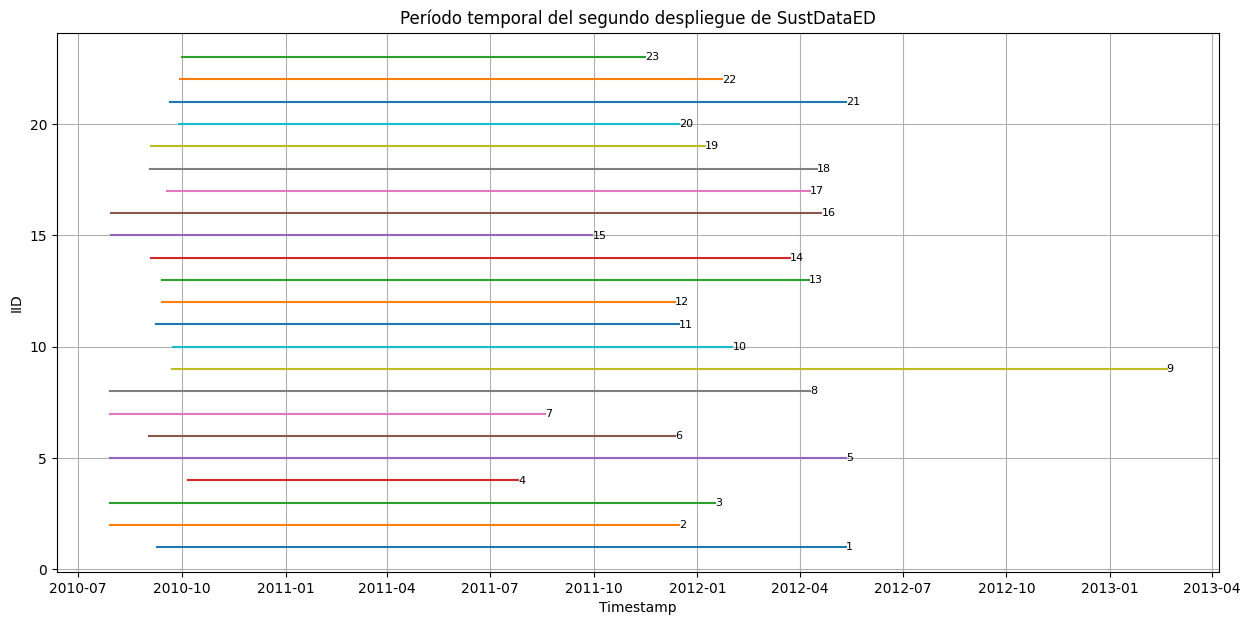
\includegraphics[width=1\textwidth,height=8cm]{img/diseno/despliegue2.png}
    \caption{Representación del período temporal que comprende el proceso de recolección de datos para cada hogar para el segundo despliegue}
    \label{fig:despliegue2}
\end{figure}

%tabla datos demographics 23 nodos





\subsubsection{Selección del rango temporal y procesamiento adicional}
\label{sec:rango}
%especificar seccion donde se comenta el rango 28-10->28-10

Como se puede ver en la Figura \ref{fig:despliegue2}, aunque las 23 viviendas pertenecen al mismo despliegue y abarcan un lapso temporal parecido, se pueden visualizar ciertas diferencias entre las mismas. Esto supone que realmente cada fichero de datos de consumo tenga un número de muestras diferente, lo que perjudicaría al análisis y entrenamiento posterior. 

\vspace{3mm}

Por tanto, una vez seleccionado el despliegue, se deben acotar los ficheros de datos de consumo a un mismo rango temporal en el se pueda trabajar de forma eficiente. Como se ha indicado anteriormente en esta misma Sección, los datos de producción energética se comienzan a medir desde el mes de octubre de 2010, por lo que es necesario como mínimo establecer el inicio del rango temporal en estas fechas. 

\vspace{3mm}

Por otro lado, entrando en el contenido de los ficheros, la fecha mínima en la que se visualiza que las 23 viviendas adquieren y almacenan medidas es el 28 de octubre de 2010, lo que lleva a tomar la decisión de establecer la misma  como inicio del rango temporal a considerar. En cuanto a la fecha final, a partir de la información dada en la Figura \ref{fig:despliegue2}, se considera que la opción más eficiente es abarcar un año completo de muestras, siendo la fecha final el 28 de octubre de 2011. En Secciones siguientes, se expondrá cómo el hecho de seleccionar un año de medidas será importante para calcular las cargas finales que se fijarán en el algoritmo \gls{den2ne} (ver Sección \ref{sec:cambiosden2ne}), puesto que en el caso de los datos de producción obtenidos de la herramienta \textit{PVWatts} se abarcan valores de potencia de un año completo (ver Sección \ref{sec:preprocpvwatts}).

\vspace{3mm}

\begin{lstlisting}[style=Python, caption={Aplicación del rango temporal a los ficheros}]
rango = df[(df['datetime'] >= '2010-10-28') & (df['datetime'] < '2011-10-28')] 
\end{lstlisting}

\vspace{3mm}

La aplicación del filtro del rango temporal a los datos se realiza en el \textit{notebook} \textit{consum\_range.ipynb}. De forma adicional, se define el procesamiento que requieren los ficheros de consumo de aquellas viviendas que no incluyen valores en algunos instantes temporales dentro del rango indicado. En este paso, el objetivo es contar con ficheros que contengan un mismo número de medidas para simplificar su manejo. Por ello, para que los datos finales tengan la mayor precisión posible, se deben añadir las muestras que faltan en función del tipo de vivienda a la que se hace referencia. 

\vspace{3mm}

Es decir, como se expuso en la Sección \ref{sec:demographic}, el dataset \textit{SustDataED} provee la Tabla \ref{tab:demo} con toda la información respectiva a cada uno de los hogares monitorizados y a las características sociales de los propios inquilinos. Esta información determina principalmente, el comportamiento eléctrico que toma cada uno de los hogares y se debe tener en cuenta para añadir las muestras necesarias a los ficheros de aquellas viviendas que tienen el rango temporal incompleto. Por ejemplo, para la vivienda con identificador 4 (ver Figura \ref{fig:despliegue2}), se deben aproximar los valores de las muestras a las proporcionadas por las viviendas con identificadores 13 o 21, puesto que la información demográfica es similar y, en consecuencia, el comportamiento eléctrico será parecido. Adicionalmente, se introduce cierto error para que los valores no sean completamente iguales entre las viviendas en cuestión.

%CODIGO





\subsection{Procesado de datos de producción}
\label{sec:procprod}

Después de exponer el procesamiento necesario para los datos de consumo, se va a profundizar en la producción energética. Como ya se había detallado en las Secciones \ref{sec:conclusionessustdata} y \ref{sec:simuprod},  referentes, respectivamente, a las conclusiones obtenidas del dataset \textit{SustDataED} y a la introducción a las herramientas de simulación de datos de producción energética, se escribe la presente Sección con el objetivo de tomar la decisión de seleccionar la fuente de datos de producción más adecuada para el desarrollo de este \gls{tfm}.

\vspace{3mm}

Por tanto, se debe comparar las características que presentan, tanto los datos que proporciona \textit{SustDataED}, como los extraídos a través de la simulación en la herramienta \textit{PVWatts}. Para ello, hay que determinar unos pasos iniciales de procesamiento en cada uno de ellos que permitan finalmente, establecer una comparación de forma correcta. En otras palabras, no sería preciso comparar ambas fuentes directamente si estas no están comprendidas en unos mismos rangos temporales o si no contienen los mismos parámetros. 

\subsubsection{Preprocesamiento de datos de \textit{SustDataED}}

En cuanto al dataset \textit{SustDataED}, el primer paso a realizar está basado en la combinación de los parámetros energéticos y los climáticos. Este viene dado por la necesidad de realizar un análisis de la correlación que existe entre la producción solar y las características ambientales que se miden en cada instante. 

\vspace{3mm}

Por ello, se crea un nuevo \textit{notebook}, denominado como \textit{preprocessing\_production.ipynb}, en el cual hay que tener en cuenta los campos expuestos en las Tablas \ref{tab:prod} y \ref{tab:env}. La operación de combinación de los datos energéticos y climáticos se determina a partir de la marca de tiempo (\textit{timestamp}) y resulta en un nuevo \textit{dataframe} de \textit{Pandas}, que será almacenado en un nuevo fichero en formato .csv.

\vspace{3mm}

\begin{lstlisting}[style=Python, caption={Combinación de ficheros}]
  df_merged = pd.merge(df_env, df_prod, on='timestamp') # Operación de merge
\end{lstlisting}

\vspace{3mm}

Posteriormente, es necesario sintetizar los datos de la misma forma que se ha realizado anteriormente para los ficheros de consumo. Como se había detallado en la Sección \ref{sec:datasamples}, se emplea el \textit{notebook} \textit{datasamples\_process.ipynb} para automatizar este proceso y obtener la media de los valores de potencia. En el caso de la producción, como este \gls{tfm} se engloba en un contexto de \gls{sg}s, se enfoca la operación en la columna de medidas globales de producción fotovoltaica. Tras la ejecución del \textit{notebook}, se obtiene un fichero con los campos definidos en la Tabla \ref{tab:prodsamples}. Adicionalmente, se emplea la librería de \textit{Python}, \textit{matplotlib}, para representar gráficamente en la Figura \ref{fig:solar} los valores de potencia recogidos en el fichero.

\vspace{3mm}

\begin{table}[h!]
  \centering
  \begin{tabular}{|c|c|c|}
  \hline
  \rowcolor[HTML]{AAAAAA} 
  \multicolumn{1}{|c|}{\cellcolor[HTML]{AAAAAA}Campo} & \multicolumn{1}{c|}{\cellcolor[HTML]{AAAAAA}Descripción} & Unidades \\ \hline
  \textit{datetime} & Fecha del valor promedio & datetime \\ \hline
  \textit{H} & Hora del valor promedio & - \\ \hline
  \textit{solar} & Electricidad producida por fuentes fotovoltaicas & MWh \\ \hline
  \end{tabular}
  \caption{Estructura de campos del fichero \textit{mean\_prod.csv}}
  \label{tab:prodsamples}
\end{table}

\vspace{3mm}

\begin{figure}[h!]
  \centering
  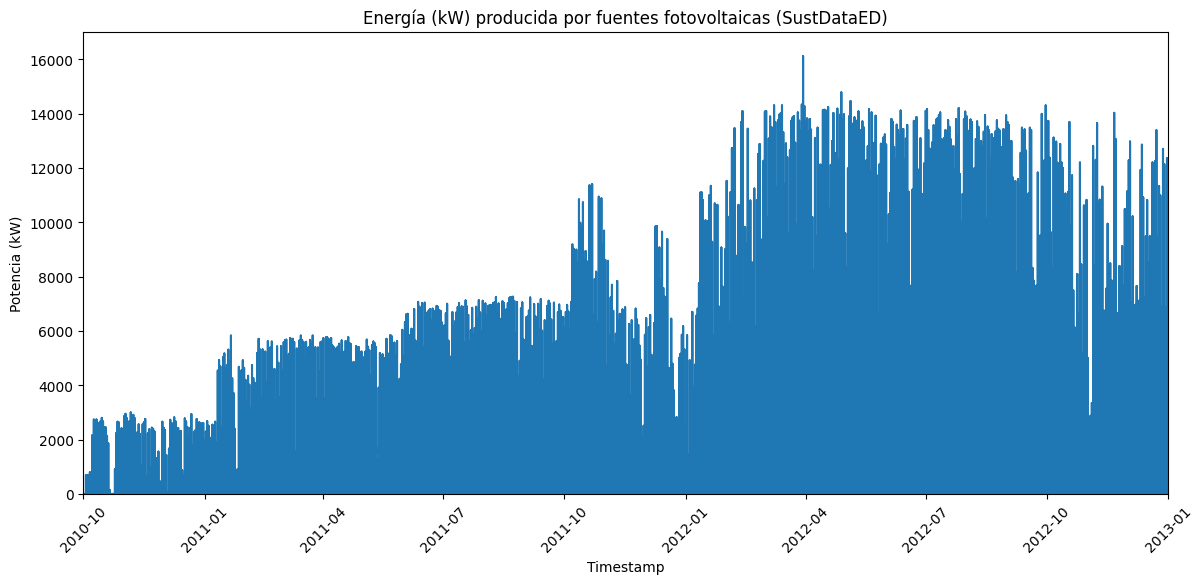
\includegraphics[width=1\textwidth]{img/diseno/matplotsolar.png}
  \caption{Gráfica de valores de energía solar producida}
  \label{fig:solar}
\end{figure}

\vspace{3mm}

De la misma forma, teniendo en cuenta el rango temporal que se ha ajustado anteriormente para los datos de consumo (ver Sección \ref{sec:rango}), se representan a modo comparativo los valores de temperatura y de potencia medidos en las Figuras \ref{fig:temp} y \ref{fig:solaryear}, respectivamente. %%%%%

\vspace{3mm}

\begin{figure}[h!]
  \centering
  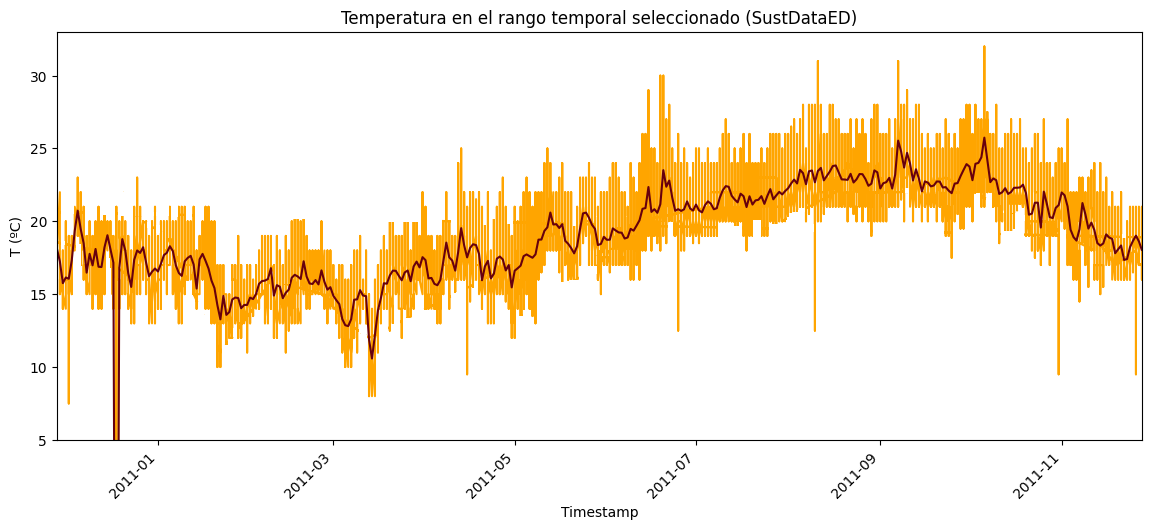
\includegraphics[width=1\textwidth]{img/diseno/temp.png}
  \caption{Gráfica de valores de temperatura en el rango seleccionado}
  \label{fig:temp}
\end{figure}

\vspace{3mm}

\begin{figure}[h!]
  \centering
  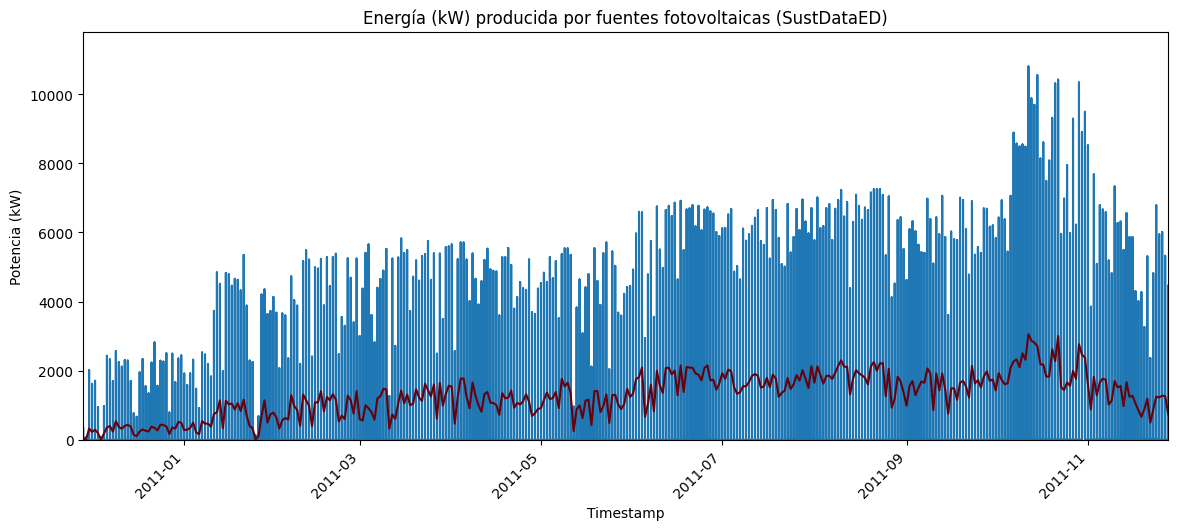
\includegraphics[width=1\textwidth]{img/diseno/matplotsolaryear.png}
  \caption{Gráfica de valores de energía solar producida en el rango seleccionado}
  \label{fig:solaryear}
\end{figure}

\subsubsection{Preprocesamiento de datos de \textit{PVWatts}}
\label{sec:preprocpvwatts}

El preprocesamiento de los datos extraídos de la herramienta \textit{PVWatts} consisten principalmente en el formateo de los mismos y en la adecuación de los valores en cada instante para el posterior cálculo de las cargas. Como motivo de esto, se añaden las operaciones necesarias en el \textit{notebook} \textit{preprocessing\_production.ipynb}. 

\vspace{3mm}

Como se había expuesto en la Sección \ref{sec:resultadossimu} y en las Tablas \ref{tab:pvwattsdataset2} y \ref{tab:pvwattsdataset}, \textit{PVWatts} proporcionaba dos datasets que replicaban un año completo de mediciones. En este caso, el preprocesamiento se va a enfocar en el que contiene las medidas adquiridas por hora para un año completo. En otros términos, como son datos simulados, no hacen referencia a un año en concreto, sino que representan valores anuales generalizados. 


Teniendo esto en cuenta, será preciso 

\vspace{3mm}



%%%%
% Preprocessing_production.ipynb 
% c.	Quitar comillas datos extraídos global data
% d.	New_pvwatts -> se añaden timestamps para crear dataset completo de producción para todas las fechas (GLOBAL). Después, se añade todo en un fichero.** 




%meter graficas del paper de sustdata
%meter graficas de sustdata (ej. consumo de un hogar y tal, correlacion prod-clima)
%definir que es lo que se va a utilizar

%ESTO ES LO QUE ESTA PUESTO ARRIBA --> (PARA ACORDARME DE REFERENCIARLO AQUI Y DETALLARLO)
% El procesamiento que será requerido para estos datos se detallará en la Sección \ref{sec:preprocesado}. No obstante, es importante destacar las características de los datos de producción eléctrica dados por \textit{SustDataED}. Como se ha expuesto anteriormente en la Sección \ref{prodsustdata}, el dataset proporciona esta información en términos globales y después, desagrega los valores energéticos según su fuente de procedencia. Como se expondrá en la Sección \ref{sec:preprocesado}, será imprescindible determinar si estos datos son precisos en un entorno de \gls{sg}s como se requiere para cumplir con los objetivos de este \gls{tfm}


% 7 y 7.1 del AI-based FDI Countermeasure for IoE Smart Grids

%hacerme una idea de la estructura -> ver pag 37 AI-based-FDI-Countermeasure-for-IoE-Smart-Grids



\subsubsection{Selección de datos de producción}
\label{sec:select}

\begin{figure}[h!]
  \centering
  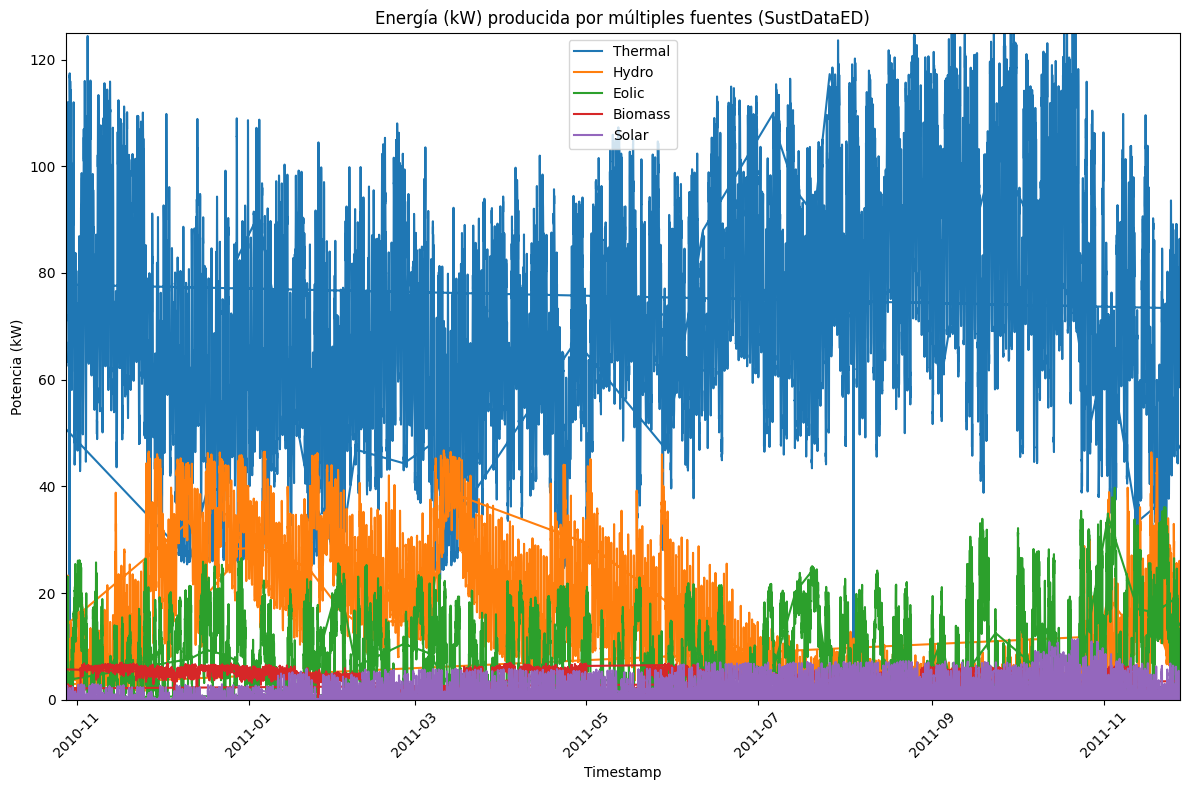
\includegraphics[width=1\textwidth]{img/diseno/matplotfuentesyear.png}
  \caption{Gráfica de valores de múltiples fuentes energéticas proporcionadas por \textit{SustDataED} para un año}
  \label{fig:fuentesyear}
\end{figure}









\subsection{Combinación de datos de consumo y de producción}
%tratamiento de nans

%meter graica consumo un nodo de ejemplos


%meter grafica load ejemplo de un nodo

